%%
%TIME NDEPENDENT: HEATMAP PLOT FOR DIFFERENT INTERPOLATING SCHEDULES
%%

\begin{figure}[ht]
  \centering
  \begin{tikzpicture}
    \begin{axis}[name=plot
    zmin=0,zmax=1,
    view={0}{90},
    colormap={inferno}{rgb255=(248,251,155) rgb255=(251,179,21) rgb255=(236,103,38) rgb255=(187,54,84) rgb255=(119,29,109) rgb255=(49,9,92) rgb255=(1,1,8)},
    colorbar,
    width = 120mm,
    height=115mm,
    xlabel = $\bm{T}$,
    ylabel = $\bm{\gamma}$
    ]
    \addplot3 [surf] table[x=a,y=b,z=c]{./Data/55_grid_linear.txt};

    \pgfplotsset{contour/every contour label/.style = {
               sloped,
               inner sep=2pt,
               transform shape,
               every node/.style={
                                 mapped color,
                                 fill=none,
                                },
              },}
    \addplot3[
            contour gnuplot=
            {
            draw color=white,
            levels={0.1, 0.2},labels=true,
            labels=true,
            contour label style={nodes={text=white}},
            handler/.style=smooth},
            contour/label distance=160pt,
            line width=1.5pt,
            contour/labels over line
           ] table [
                    x =a,
                    y = b,
                    z = c,
                   ]{./Data/55_grid_linear.txt};

    \end{axis}
  \end{tikzpicture}
\end{figure}


\begin{figure}[ht]
\centering
\begin{tabular}{cc}
  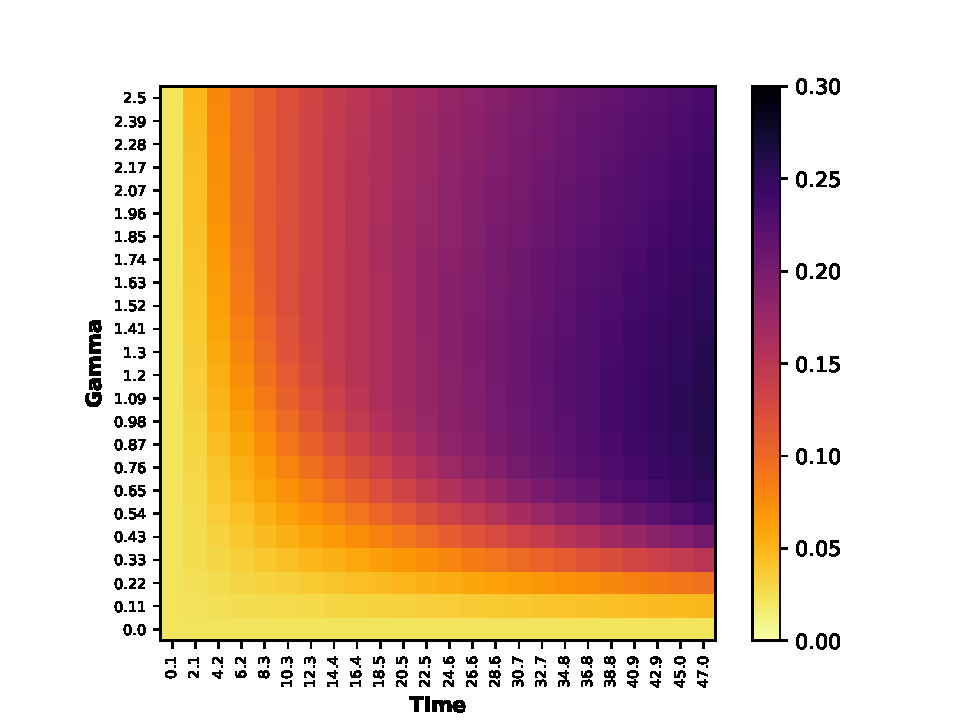
\includegraphics[width=75mm]{./figures/time_dependent_heatmap/47_heatmap_time_dependent_lin.pdf} &   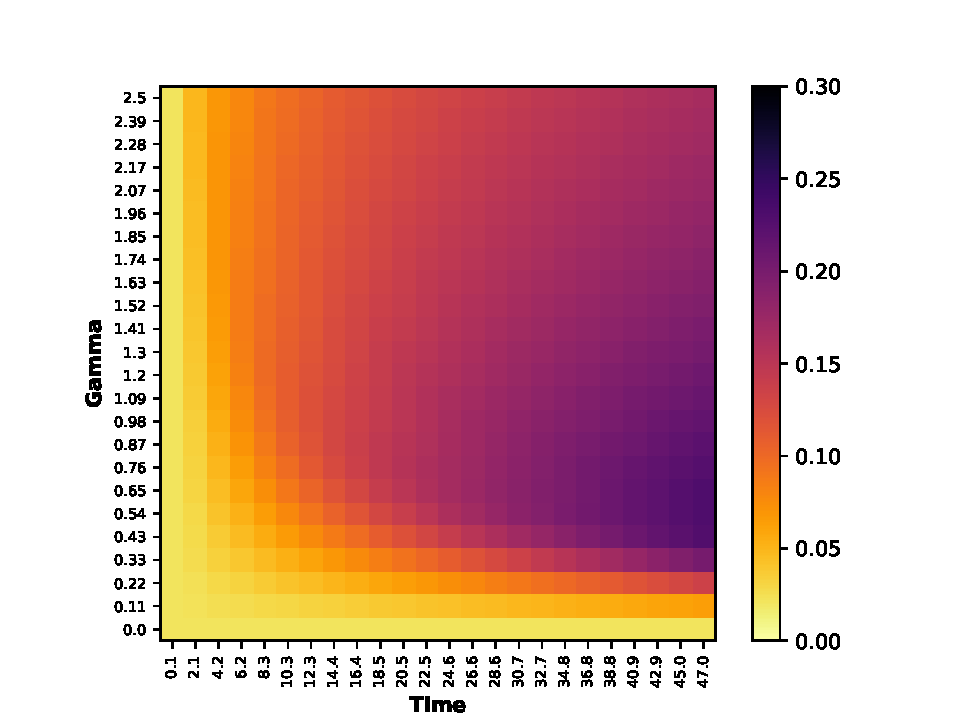
\includegraphics[width=75mm]{./figures/time_dependent_heatmap/47_heatmap_time_dependent_sqrt.pdf} \\
(a) lin & (b) sqrt\\[6pt]
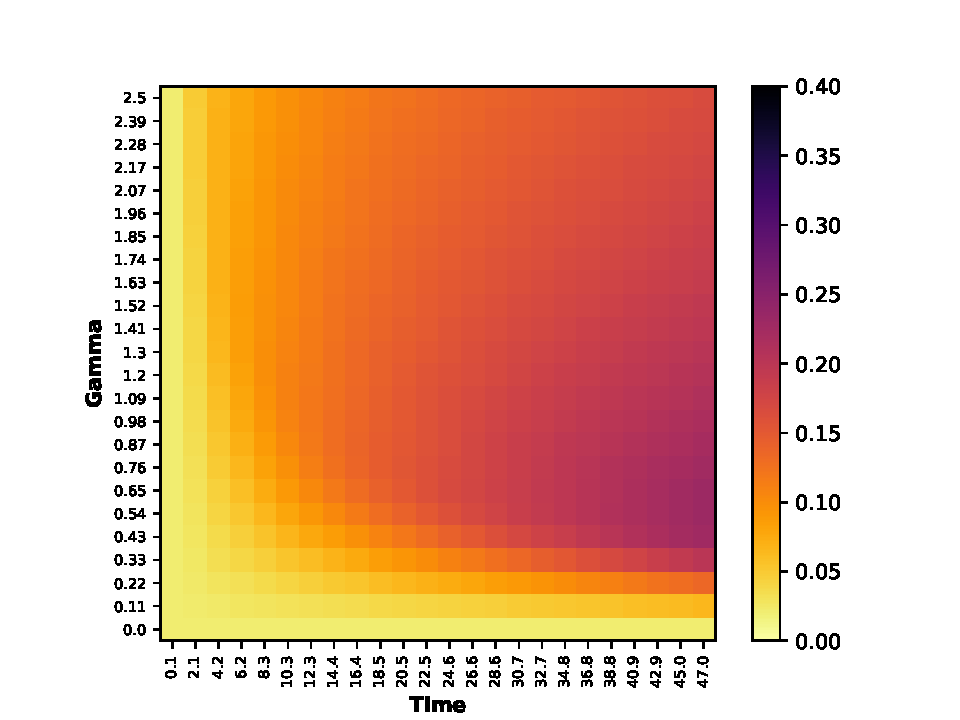
\includegraphics[width=75mm]{./figures/time_dependent_heatmap/47_heatmap_time_dependent_cbrt.pdf} &   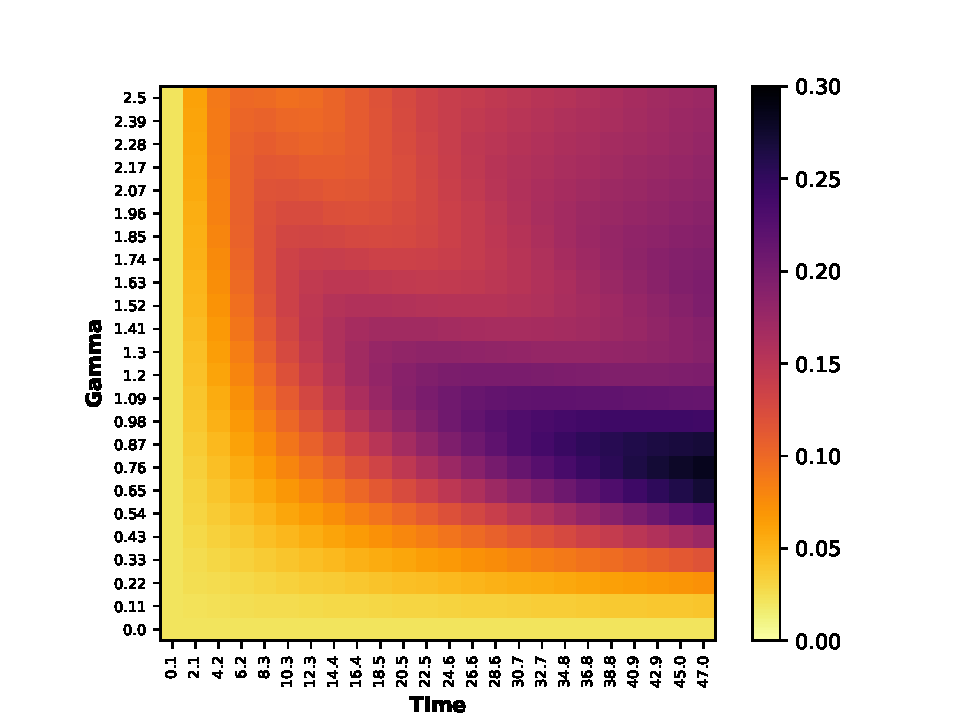
\includegraphics[width=75mm]{./figures/time_dependent_heatmap/47_heatmap_time_dependent_cerf.pdf} \\
(c) cbrt & (d) cerf\\[6pt]
\end{tabular}
\caption[Probability heatmap plot for the time-dependent Hamiltonian, for different shapes of s(t)]{\textbf{Probability heatmap plot for the time-dependent Hamiltonian, for different shapes of s(t).} The figure shows the probability distribution for a circular graph of N=47 evaluated using the time-dependent Hamiltonian using the following interpolating schedules (a) linear, (b) $\sqrt{t/T}$, (c) $\sqrt[3]{t/T}$ and (d) Roland-Cerf(3). Note that the color gradient is normalized to p=0.3 to accentuate the difference in probability between different regions. }
\label{fig:heatmap-dependent}
\end{figure}
